\documentclass[journal]{IEEEtran}

\usepackage{amsmath,amssymb,amsthm}
\usepackage{booktabs}
\usepackage{array}
\usepackage{graphicx}
\usepackage{pgfplots,pgfplotstable}
\usepgfplotslibrary{groupplots}
\usepackage{tikz}
\pgfplotsset{compat=1.18}
\usepackage{cite}
\usepackage{url}
\usepackage[hidelinks]{hyperref}
\usepackage{microtype}
\usepackage{placeins}

\newtheorem{theorem}{Theorem}
\newtheorem{corollary}{Corollary}
\newtheorem{proposition}{Proposition}
\newtheorem{remark}{Remark}

\newcommand{\Pone}{\mathbb{P}_1}
\newcommand{\Pzero}{\mathbb{P}_0}
\newcommand{\Eone}{\mathbb{E}_1}
\newcommand{\Ezero}{\mathbb{E}_0}
\newcommand{\LR}{\Lambda}
\newcommand{\ind}{\mathbf{1}}

\title{Boundary-Localized Genomic Utility and Clinical-Tail Dominance:\\
A Likelihood-Ratio Theory for ZeBRA and Fibrotic Interstitial Lung Disease}

\author{Ishanu Chattopadhyay\\
Division of Biomedical Informatics, University of Kentucky College of Medicine}

\begin{document}
\maketitle

\begin{abstract}
Genomic risk and longitudinal clinical history are distinct information channels for forecasting future disease. We study when a static germline genomic channel can add predictive value once a longitudinal clinical-history score has become strongly informative. The central object is the residual genomic likelihood ratio conditional on clinical history. If this residual genomic evidence is uniformly bounded while sequential clinical evidence can develop an extended likelihood-ratio tail, then two consequences follow. First, genomic information can change a likelihood-ratio decision only inside a bounded neighborhood of the clinical decision threshold; outside that region the clinical evidence is already too strong for bounded genomic evidence to reverse the decision. Second, at sufficiently extreme specificity, the clinical likelihood-ratio test strictly dominates every genomic-only rule whose likelihood ratio is bounded. We also show that any deterministic genomic model inherits the bound and that decision-local benefit can coexist with negligible global AUC change. We evaluate these predictions in a Colorado fibrotic interstitial lung disease (ILD) analysis using ZeBRA, a longitudinal EHR-derived score, and a curated genomic panel containing \textit{MUC5B} rs35705950. Across repeated held-out splits, ZeBRA dominates global discrimination, broad genomic augmentation provides essentially no global FILD/FILA gain after conditioning on ZeBRA, and ZeBRA predicts \textit{MUC5B} carrier status only at chance level. Nevertheless, \textit{MUC5B} retains significant conditional disease information in restricted ZeBRA operating bands, and a two-threshold genomic rescue rule increases held-out sensitivity by up to approximately 4.5 percentage points at essentially matched false-positive rate. The empirical pattern is therefore not global genomic redundancy but regime-dependent complementarity localized near the clinical decision boundary.
\end{abstract}

\begin{IEEEkeywords}
ZeBRA, fibrotic interstitial lung disease, idiopathic pulmonary fibrosis, MUC5B, genomics, likelihood ratio, Neyman--Pearson lemma, Bayesian inference, decision boundary.
\end{IEEEkeywords}

\section{Motivating problem: ZeBRA and genomic risk in fibrotic ILD}

Fibrotic ILDs, including idiopathic pulmonary fibrosis (IPF), have a strong but non-Mendelian genetic component. The \textit{MUC5B} promoter variant rs35705950 is among the strongest common genetic risk factors for pulmonary fibrosis \cite{Seibold2011,Fingerlin2013,Allen2020}. In the original report, the minor allele was present much more frequently among subjects with IPF than among controls \cite{Seibold2011}. At the same time, disease emergence is accompanied by a growing sequence of clinically observable diagnoses, prescriptions, procedures, and comorbidities. ZeBRA is designed to summarize such routinely observed longitudinal clinical histories into a future-risk score without requiring laboratory tests, imaging, or questionnaires \cite{Onishchenko2026}.

Our recent fibrotic ILD analyses ask whether genomic information improves prediction once ZeBRA is known. In 30 repeated held-out splits of the current operational FILD/FILA endpoint, mean AUC is approximately 0.814 for ZeBRA, 0.566 for the selected genomic panel, and 0.799 for a nonlinear combined model. Because that comparison alone does not isolate incremental information, we also performed a paired regularized analysis in which ZeBRA-only and ZeBRA-plus-genomics models were evaluated on the same held-out subjects. For FILD/FILA, the mean paired AUC increment from the complete genomic panel is only $+0.00043$, the median increment is 0, and the split-wise 2.5th--97.5th percentile range spans approximately $-0.0051$ to $+0.0041$; average precision decreases and both Brier score and log loss worsen after broad genomic augmentation.

The absence of global gain is not explained by ZeBRA reconstructing the major genomic signal. Among subjects with called rs35705950 genotype, ZeBRA predicts \textit{MUC5B} carrier status at chance level (AUC approximately 0.509). A modest pooled enrichment of carriers in the extreme ZeBRA tail disappears after stratification by FILD/FILA status, showing that the pooled association is consistent with both channels tracking disease rather than with clinical history encoding genotype. Yet residual \textit{MUC5B} disease information is strongly heterogeneous across ZeBRA score space. In the ZeBRA band corresponding approximately to 5--10\% control FPR, adding \textit{MUC5B} after ZeBRA yields a likelihood-ratio statistic of 16.55 ($p\approx4.7\times10^{-5}$). A two-threshold rule that consults \textit{MUC5B} only between a stringent upper and lower ZeBRA threshold increases held-out sensitivity by up to approximately 4.5 percentage points while preserving essentially the same realized overall FPR. These observations motivate and correspond to the theory below; they are not taken as proofs of its regularity assumptions.

The apparent paradox is therefore:
\begin{quote}
A strong genomic risk factor can be biologically important, and can improve decisions for selected individuals, while contributing almost nothing to global discrimination once a strong clinical-history predictor is available.
\end{quote}

We show that this behavior is expected under a general Bayesian likelihood-ratio formulation.

\section{Latent-state and information-channel formulation}

Let $B_t$ denote the latent biological state at time $t$, $G$ the germline genomic state, and $E_{0:t}$ the accumulated non-genetic exposure history. The biological state evolves under the influence of $G$ and $E_{0:t}$. For a fixed future horizon $h>0$, define the disease-risk functional
\begin{equation}
\rho_h(B_t)
=\mathbb{P}(T\le t+h\mid T>t,B_t),
\label{eq:rho}
\end{equation}
where $T$ is the disease-event time. The clinical event sequence $C_{0:t}$ is a noisy observation of the latent biological trajectory $B_{0:t}$. In the idealized Bayesian limit, a clinical-history predictor satisfies
\begin{equation}
Z_h(C_{0:t})
=\mathbb{P}(T\le t+h\mid C_{0:t})
=\int \rho_h(b)\,d\mathbb{P}(B_t=b\mid C_{0:t}).
\label{eq:zposterior}
\end{equation}
Thus ZeBRA need not reconstruct $B_t$; it estimates the disease-relevant functional of $B_t$ from the clinical observation channel.

For the theorem it is enough to reduce the problem to binary prediction. Let
\begin{equation}
Y=\ind\{T\le t+h\}\in\{0,1\},
\end{equation}
and write $C$ for the available clinical history. The genomic channel $G$ and clinical channel $C$ are then placed on equal statistical footing through their disease-versus-control likelihood ratios.

\section{Likelihood-ratio representation}

Let $\Pone(\cdot)=\mathbb{P}(\cdot\mid Y=1)$ and $\Pzero(\cdot)=\mathbb{P}(\cdot\mid Y=0)$. Assume the relevant distributions admit densities with respect to common dominating measures. Define the clinical likelihood ratio
\begin{equation}
\LR_C(c)=\frac{p(c\mid Y=1)}{p(c\mid Y=0)},
\label{eq:clinicalLR}
\end{equation}
and the residual genomic likelihood ratio conditional on clinical history
\begin{equation}
\LR_{G\mid C}(g;c)
=\frac{p(g\mid Y=1,C=c)}{p(g\mid Y=0,C=c)}.
\label{eq:conditionalGLR}
\end{equation}
The full joint likelihood ratio is
\begin{equation}
\LR_{C,G}(c,g)
=\frac{p(c,g\mid Y=1)}{p(c,g\mid Y=0)}.
\end{equation}
By the probability chain rule,
\begin{equation}
\boxed{
\LR_{C,G}(c,g)
=\LR_C(c)\,\LR_{G\mid C}(g;c).
}
\label{eq:factorization}
\end{equation}
No conditional-independence assumption is required.

If $Z$ is a calibrated clinical posterior, $Z=\mathbb{P}(Y=1\mid C)$, and $\pi=\mathbb{P}(Y=1)$, Bayes' rule yields
\begin{equation}
\frac{Z}{1-Z}
=\frac{\pi}{1-\pi}\LR_C(C),
\label{eq:zlr}
\end{equation}
so thresholding calibrated ZeBRA is equivalent to thresholding $\LR_C$. More generally, the same results apply whenever the clinical score is a strictly monotone transformation of $\LR_C$.

\section{Main theorem}

The key biological assumptions are deliberately weak.

\textbf{A1 (Uniformly bounded residual genomic evidence).} There exist constants $0<m\le 1\le M<\infty$ such that
\begin{equation}
0<m\le \LR_{G\mid C}(g;c)\le M<\infty
\label{eq:boundedconditional}
\end{equation}
for the relevant support of $(g,c)$, and the marginal genomic likelihood ratio
\begin{equation}
\LR_G(g)=\frac{p(g\mid Y=1)}{p(g\mid Y=0)}
\end{equation}
is bounded above by $M_G<\infty$. Complex, non-Mendelian disease architecture motivates finite residual genomic Bayes factors, but does not by itself imply a uniform bound over all conditioned clinical states; boundedness is therefore an explicit regularity assumption.

\textbf{A2 (Accumulating clinical evidence).} Clinical history is sequential, $C_n=(X_1,\ldots,X_n)$, and continued diagnoses, prescriptions, procedures, and comorbidities can produce an extended disease-evidence tail. Formally, $\LR_C$ is not bounded above on the relevant sequence of clinical histories: for arbitrarily large $K$ there are events with positive $\Pzero$ probability on which $\LR_C\ge K$.

\begin{theorem}[Boundary-localized genomic utility and clinical-tail dominance]
\label{thm:main}
Under A1--A2:

\emph{(i) Exact factorization.} The optimal joint disease-versus-control likelihood ratio is
\begin{equation}
\LR_{C,G}=\LR_C\LR_{G\mid C}.
\end{equation}

\emph{(ii) Boundary localization.} For any likelihood-ratio decision threshold $\lambda>0$, genomic information can change which side of the threshold an observation occupies only if
\begin{equation}
\boxed{
\frac{\lambda}{M}
\le \LR_C(c)
\le \frac{\lambda}{m}.
}
\label{eq:boundaryband}
\end{equation}
Equivalently,
\begin{equation}
\boxed{
-\log M
\le
\log \LR_C(c)-\log\lambda
\le
-\log m.
}
\label{eq:logboundaryband}
\end{equation}
Hence the genomic decision-relevant region has fixed width
\begin{equation}
\log(M/m)
\end{equation}
on the clinical log-likelihood scale, independent of where the decision boundary $\lambda$ is placed.

\emph{(iii) Genomic-only power is bounded.} For any test $\phi(G)\in[0,1]$ using genomics alone, with false-positive rate $\alpha=\Ezero[\phi(G)]$, its true-positive rate satisfies
\begin{equation}
\boxed{
\Eone[\phi(G)]\le M_G\alpha.
}
\label{eq:genomicpowerbound}
\end{equation}
Thus the positive likelihood ratio of any genomic-only decision rule is at most $M_G$.

\emph{(iv) Clinical superiority at extreme specificity.} For any $K>M_G$ with $\alpha_K=\Pzero(\LR_C\ge K)>0$, the clinical likelihood-ratio test
\begin{equation}
\phi_K(C)=\ind\{\LR_C(C)\ge K\}
\end{equation}
has
\begin{equation}
\frac{\Pone(\LR_C\ge K)}{\Pzero(\LR_C\ge K)}\ge K>M_G.
\label{eq:clinicalLRplus}
\end{equation}
Therefore, at the same FPR $\alpha_K$, its power is strictly greater than that of every genomic-only test. Moreover,
\begin{equation}
\alpha_K\le \frac{1}{K}\to0
\end{equation}
as $K\to\infty$. Hence the superiority occurs in the extreme-specificity limit.

\emph{(v) Clinical-tail dominance in the combined evidence.} Along sequences with $\LR_C\to\infty$,
\begin{equation}
\log \LR_{C,G}
=\log \LR_C+O(1),
\end{equation}
and therefore
\begin{equation}
\boxed{
\frac{\log\LR_{C,G}}{\log\LR_C}\to1.
}
\label{eq:taildominance}
\end{equation}
Thus bounded genomic evidence is asymptotically negligible relative to the accumulated clinical log-likelihood in the extreme clinical-evidence tail.
\end{theorem}

\begin{proof}
Part (i) is the chain rule:
\begin{align}
\LR_{C,G}(c,g)
&=\frac{p(c,g\mid Y=1)}{p(c,g\mid Y=0)}\\
&=\frac{p(c\mid Y=1)p(g\mid Y=1,c)}
        {p(c\mid Y=0)p(g\mid Y=0,c)}\\
&=\LR_C(c)\LR_{G\mid C}(g;c).
\end{align}

For part (ii), compare the clinical-only decision $\LR_C\ge\lambda$ with the joint decision $\LR_C\LR_{G\mid C}\ge\lambda$. If
\begin{equation}
\LR_C<\lambda/M,
\end{equation}
then A1 gives
\begin{equation}
\LR_C\LR_{G\mid C}
\le \LR_C M
<\lambda,
\end{equation}
so no genomic state can move the observation above the threshold. Conversely, if
\begin{equation}
\LR_C>\lambda/m,
\end{equation}
then
\begin{equation}
\LR_C\LR_{G\mid C}
\ge \LR_C m
>\lambda,
\end{equation}
so no genomic state can move the observation below the threshold. Hence a threshold change is possible only on the interval in \eqref{eq:boundaryband}. Taking logarithms gives \eqref{eq:logboundaryband}; its width is
\begin{equation}
(-\log m)-(-\log M)=\log(M/m),
\end{equation}
which does not depend on $\lambda$.

For part (iii), let $\phi(G)\in[0,1]$. Using the Radon--Nikodym identity under $\Pzero$,
\begin{align}
\Eone[\phi(G)]
&=\Ezero[\LR_G(G)\phi(G)]\\
&\le M_G\Ezero[\phi(G)]\\
&=M_G\alpha.
\end{align}
This proves \eqref{eq:genomicpowerbound}. The result holds for randomized as well as deterministic genomic rules.

For part (iv), define $A_K=\{c:\LR_C(c)\ge K\}$. Then
\begin{align}
\Pone(A_K)
&=\Ezero[\LR_C(C)\ind\{A_K\}]\\
&\ge K\Ezero[\ind\{A_K\}]\\
&=K\Pzero(A_K)\\
&=K\alpha_K.
\end{align}
Therefore the clinical rule has LR$+$ at least $K$. If $K>M_G$, any genomic-only test with the same FPR $\alpha_K$ has power at most $M_G\alpha_K<K\alpha_K\le\Pone(A_K)$. By the Neyman--Pearson lemma \cite{NeymanPearson1933}, thresholding $\LR_C$ is also the most powerful rule among all tests measurable with respect to $C$ at the corresponding size (with the usual boundary randomization if needed).

Finally, because $\Ezero[\LR_C]=1$, Markov's inequality gives
\begin{equation}
\alpha_K
=\Pzero(\LR_C\ge K)
\le\frac{\Ezero[\LR_C]}{K}
=\frac{1}{K},
\end{equation}
so $\alpha_K\to0$ as $K\to\infty$. This is precisely the high-specificity regime.

For part (v), A1 implies
\begin{equation}
\log m\le\log\LR_{G\mid C}\le\log M,
\end{equation}
so $\log\LR_{G\mid C}=O(1)$. By part (i),
\begin{equation}
\log\LR_{C,G}
=\log\LR_C+\log\LR_{G\mid C}
=\log\LR_C+O(1).
\end{equation}
Dividing by $\log\LR_C$ and letting $\LR_C\to\infty$ yields \eqref{eq:taildominance}.
\end{proof}

\begin{corollary}[Posterior-risk form for ZeBRA]
\label{cor:zebra}
If ZeBRA is calibrated so that $Z=\mathbb{P}(Y=1\mid C)$, let $\tau\in(0,1)$ be any ZeBRA decision threshold and define posterior-odds threshold $\kappa=\tau/(1-\tau)$. Then genomic information can change the decision only if
\begin{equation}
\boxed{
\frac{\kappa}{M}
\le
\frac{Z}{1-Z}
\le
\frac{\kappa}{m}.
}
\label{eq:zboundary}
\end{equation}
Equivalently,
\begin{equation}
-\log M
\le
\operatorname{logit}(Z)-\operatorname{logit}(\tau)
\le
-\log m.
\end{equation}
Thus genomic utility is localized around \emph{whatever} ZeBRA operating boundary is chosen.
\end{corollary}

\begin{proof}
Equation \eqref{eq:zlr} shows that ZeBRA posterior odds differ from $\LR_C$ by the positive constant prior odds $\pi/(1-\pi)$. Substitution into Theorem~\ref{thm:main}(ii) yields the result.
\end{proof}

\begin{corollary}[Any genomic model inherits the bound]
Let $S=f(G)$ be any measurable genomic predictor, including a polygenic risk score, gradient-boosted model, random forest, neural network, or generative genomic model. If the full genomic likelihood ratio is bounded, then the likelihood ratio of $S$ is also bounded. Therefore no deterministic compression or machine-learning transformation of the same genomic information can evade the finite-evidence and extreme-specificity conclusions of Theorem~\ref{thm:main}.
\end{corollary}

\begin{proof}
For a score value $s$, the score likelihood ratio can be written as a conditional average of the full genomic likelihood ratio under $\Pzero$:
\begin{equation}
\LR_S(s)
=\mathbb{E}_0[\LR_G(G)\mid S=s].
\end{equation}
A conditional expectation of a random variable bounded above by $M_G$ is itself bounded above by $M_G$. The analogous lower bound follows if $\LR_G$ is bounded away from zero.
\end{proof}

\begin{proposition}[Local decision gain can coexist with negligible global AUC change]
\label{prop:auc-local}
Let $S(C)$ be a clinical score and $S'(C,G)$ an augmented score. Suppose $S'=S$ except on a measurable region $B$ of the clinical--genomic state space. Then
\begin{align}
\left|\operatorname{AUC}(S')-\operatorname{AUC}(S)\right|
&\le \Pone(B)+\Pzero(B)-\Pone(B)\Pzero(B)\\
&\le \Pone(B)+\Pzero(B).
\label{eq:auc-local-bound}
\end{align}
Hence an augmented rule can produce a substantial change in decisions within a small boundary region while producing an arbitrarily small change in global AUC as the case and control mass of that region tends to zero.
\end{proposition}

\begin{proof}
AUC is the probability that a randomly drawn case receives a higher score than a randomly drawn control, with the usual half-credit convention for ties. If neither member of a case--control pair lies in $B$, then $S'=S$ for both members and the pairwise ranking contribution is unchanged. Therefore the AUC contribution can differ only when at least one member of the pair lies in $B$. The probability of that event is
\begin{align}
&1-(1-\Pone(B))(1-\Pzero(B))\\
&\qquad=\Pone(B)+\Pzero(B)-\Pone(B)\Pzero(B),
\end{align}
which bounds the maximum possible AUC change.
\end{proof}

\section{Why the clinical channel can have an extended tail}

The theorem does not assume that every later clinical event is informative, nor that disease becomes perfectly observable. It requires only that the clinical channel can accumulate sufficiently strong evidence on some disease trajectories. For a sequential history $C_n=(X_1,\ldots,X_n)$, the clinical likelihood ratio factorizes exactly as
\begin{equation}
\LR_C(C_n)
=\prod_{k=1}^{n}
\frac{p(X_k\mid Y=1,X_{<k})}
     {p(X_k\mid Y=0,X_{<k})},
\label{eq:sequentialLR}
\end{equation}
so that
\begin{equation}
\log\LR_C(C_n)
=\sum_{k=1}^{n}
\log
\frac{p(X_k\mid Y=1,X_{<k})}
     {p(X_k\mid Y=0,X_{<k})}.
\label{eq:sequentiallogLR}
\end{equation}
This is the standard likelihood-ratio accumulation underlying sequential testing \cite{Wald1945}. The genomic state does not acquire new germline variants as the disease approaches, whereas the clinical history can acquire additional diagnoses, procedures, prescriptions, and comorbidities. The difference is therefore not that clinical and genomic predictors obey different probability laws; both enter Bayes' rule as evidence. The difference is that one channel is static and finite while the other is longitudinal and can supply repeated likelihood-ratio factors.

Equation \eqref{eq:sequentialLR} also clarifies the sense in which clinical odds may rise sharply: likelihood evidence adds in log space but multiplies in odds space. No claim of exponential growth follows from AUC alone. Rather, when a sequence contains repeated positive log-likelihood increments, the posterior odds are the exponential of their accumulated sum.

\section{Interpretation of the theoretical result}

The theorem and Proposition~\ref{prop:auc-local} make four distinct claims that should not be conflated.

\subsection{Global discrimination is not the quantity controlled by the theorem}
Theorem~\ref{thm:main}(ii) is about whether bounded residual genomic evidence can change a threshold decision, not about global ranking. If genomic information matters only in the boundary band \eqref{eq:boundaryband}, then only a restricted fraction of case--control pairs can be reordered. Proposition~\ref{prop:auc-local} formalizes the consequence: a meaningful local operating-point improvement can coexist with a negligible global AUC change. Thus ``no AUC gain'' and ``local genomic utility'' are mathematically compatible rather than contradictory.

\subsection{Weak ZeBRA--genotype association does not imply zero conditional genomic disease information}
The relevant residual quantity is $\LR_{G\mid C}$, not the marginal dependence between the clinical score and genotype. ZeBRA can be nearly uninformative about rs35705950 carrier status while \textit{MUC5B} still changes disease odds conditional on a particular clinical state. The channels can therefore be statistically distinct yet jointly useful near selected boundaries.

\subsection{Decision utility is expected to move with the operating threshold}
Corollary~\ref{cor:zebra} shows that the genomic decision-relevant region is defined relative to the chosen ZeBRA threshold. There is no unique genomic ``useful band'' independent of the decision problem. Changing the tolerated false-positive rate changes the clinical boundary and therefore changes which patients can be reclassified by bounded genomic evidence.

\subsection{Clinical-tail dominance is a high-specificity statement, not an AUC statement}
Theorem~\ref{thm:main}(iii)--(v) concerns the likelihood-ratio tail. A genomic-only rule has LR$+$ bounded by $M_G$, whereas a sufficiently extreme clinical likelihood-ratio threshold has LR$+$ at least $K$ with FPR at most $1/K$. The empirical quantities most relevant to this part of the theory are therefore stringent-specificity likelihood ratios and low-FPR operating behavior, not global AUC by itself.

\section{Empirical correspondence in the Colorado ILD analysis}
\label{sec:empirical}

\subsection{Cohort and analysis hierarchy}
The current analysis uses the Colorado genomic--clinical cohort assembled in \texttt{zebra\_comp}. Three stored phenotype fields are evaluated: \texttt{FILD or FILA ADJUDICATED}, \texttt{NONFIBROTIC ILD ADJUDICATED}, and \texttt{NON FIBROTIC ILA ADJUDICATED}. The historical notebook construction maps \texttt{Y/y} to 1 and \texttt{N/n} to 0, converts the field to numeric, assigns missing target values to 0, and excludes observations without an available 104-week ZeBRA score. The reported endpoint is therefore the notebook-defined operational target; not every target-zero observation is an independently adjudicated negative. This distinction matters especially when interpreting FPR.

The empirical analyses are intentionally hierarchical. Notebook~32 asks whether genomics alone or broad nonlinear ZeBRA+genomics improves global held-out discrimination. Notebook~33 asks the more specific paired question of incremental genomic value conditional on ZeBRA. Separate analyses then test whether ZeBRA reconstructs \textit{MUC5B}, where residual \textit{MUC5B} information lies in ZeBRA score space, and whether a two-threshold genomic rule improves boundary decisions at matched FPR.

\begin{table*}[!t]
\caption{Theory--evidence correspondence. The empirical analyses illustrate predicted consequences; they do not prove A1 or A2.}
\label{tab:theory-evidence-map}
\centering\footnotesize\setlength{\tabcolsep}{5pt}
\begin{tabular}{p{0.23\textwidth}p{0.31\textwidth}p{0.37\textwidth}}
\toprule
Theory & Analysis & Empirical meaning\\
\midrule
Distinct channels and residual genomic evidence & ZeBRA-to-\textit{MUC5B} pooled and FILD-stratified analyses & Weak global genomic increment is not explained by ZeBRA reconstructing genotype.\\
Boundary localization, Theorem~\ref{thm:main}(ii) & Local ZeBRA--\textit{MUC5B} information curves and FPR-defined bands & Conditional genomic disease information is heterogeneous across clinical-score space.\\
Local gain with little global AUC change, Proposition~\ref{prop:auc-local} & Notebook~32 and notebook~33 plus matched-FPR rescue & Global augmentation yields essentially no FILD AUC gain even though selected boundary decisions improve.\\
Clinical-tail dominance, Theorem~\ref{thm:main}(iii)--(v) & Low-FPR sensitivity and LR$+$ behavior & Stringent clinical operating points can dominate genomic-only evidence even when genomics remains locally useful.\\
\bottomrule
\end{tabular}
\end{table*}

\pgfplotstableread[col sep=comma]{data/global_auc_summary.csv}\globalauc
\pgfplotstableread[col sep=comma]{data/incremental_summary.csv}\incremental
\pgfplotstableread[col sep=comma]{data/local_info_bands.csv}\localbands
\pgfplotstableread[col sep=comma]{data/boundary_rescue_summary_ordered_ext.csv}\rescuedata
\pgfplotstableread[col sep=comma]{data/low_fpr_operating_points.csv}\lowfprdata
\pgfplotstableread[col sep=comma]{data/low_fpr_upper_envelope.csv}\lowenv

\subsection{Global repeated-split discrimination}
Across 30 repeated held-out outer splits, ZeBRA is the strongest predictor for all three endpoints. For FILD/FILA, mean AUC is 0.8142 for ZeBRA, 0.5662 for genomics alone, and 0.7988 for the nonlinear combined model. The same qualitative ordering is stronger for the two nonfibrotic endpoints. These results establish the global pattern, but do not by themselves test whether genomics has a small conditional increment after ZeBRA is known.

\begin{figure*}[!t]
\centering
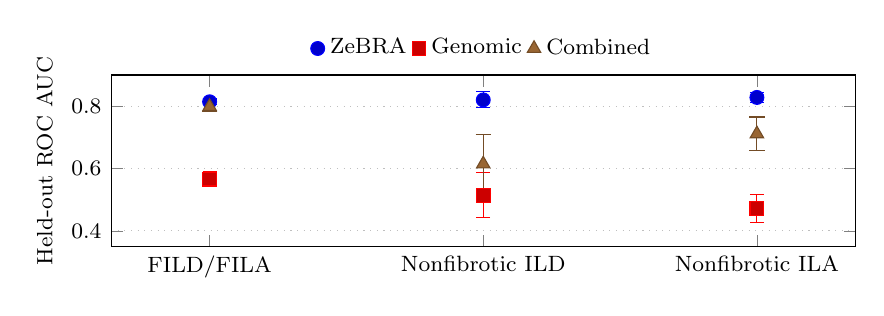
\begin{tikzpicture}
\begin{axis}[width=0.91\textwidth,height=0.31\textwidth,
ylabel={Held-out ROC AUC},ymin=0.35,ymax=0.90,
xtick={0,1,2},xticklabels={FILD/FILA,Nonfibrotic ILD,Nonfibrotic ILA},
xticklabel style={font=\footnotesize},yticklabel style={font=\footnotesize},label style={font=\footnotesize},
legend style={at={(0.5,1.03)},anchor=south,legend columns=3,draw=none,font=\footnotesize},
ymajorgrids=true,major grid style={dotted},enlarge x limits=0.18]
\addplot+[only marks,mark=*,mark size=2.5pt,error bars/.cd,y dir=both,y explicit] coordinates {(0,0.8142)+-(0,0.0089) (1,0.8202)+-(0,0.0257) (2,0.8281)+-(0,0.0162)};\addlegendentry{ZeBRA}
\addplot+[only marks,mark=square*,mark size=2.5pt,error bars/.cd,y dir=both,y explicit] coordinates {(0,0.5662)+-(0,0.0245) (1,0.5141)+-(0,0.0719) (2,0.4717)+-(0,0.0443)};\addlegendentry{Genomic}
\addplot+[only marks,mark=triangle*,mark size=2.8pt,error bars/.cd,y dir=both,y explicit] coordinates {(0,0.7988)+-(0,0.0150) (1,0.6145)+-(0,0.0953) (2,0.7112)+-(0,0.0541)};\addlegendentry{Combined}
\end{axis}\end{tikzpicture}
\caption{Global repeated-split discrimination from notebook~32. Points are mean held-out AUC over 30 outer splits; bars indicate one standard deviation. The clinical-history channel dominates globally, and broad nonlinear combination does not improve ZeBRA.}
\label{fig:global-auc}
\end{figure*}

\begin{table*}[!t]
\caption{Held-out AUC over 30 repeated outer splits from notebook~32. Values are mean $\pm$ SD.}
\label{tab:auc-repeated}\centering\footnotesize
\begin{tabular}{lccc}\toprule
Target & ZeBRA & Genomic & Combined\\\midrule
FILD/FILA & $0.8142\pm0.0089$ & $0.5662\pm0.0245$ & $0.7988\pm0.0150$\\
Nonfibrotic ILD & $0.8202\pm0.0257$ & $0.5141\pm0.0719$ & $0.6145\pm0.0953$\\
Nonfibrotic ILA & $0.8281\pm0.0162$ & $0.4717\pm0.0443$ & $0.7112\pm0.0541$\\\bottomrule
\end{tabular}
\end{table*}

\subsection{Paired incremental value conditional on ZeBRA}
Notebook~33 evaluates ZeBRA-only and ZeBRA-plus-genomics models on the same held-out subjects in 30 repeated splits. For FILD/FILA, the mean paired AUC difference is only $+0.00043$, the median is 0, and the split-wise 2.5th--97.5th percentile interval is $[-0.00507,0.00408]$. Average precision decreases, while Brier score and log loss worsen. The conclusion is therefore not merely that one nonlinear combined model underperformed, but that broad genomic augmentation supplies no reproducible global FILD/FILA discrimination gain conditional on ZeBRA.

\begin{figure*}[!t]
\centering
\begin{tikzpicture}
\begin{groupplot}[group style={group size=2 by 1,horizontal sep=1.45cm},width=0.43\textwidth,height=0.28\textwidth,
tick label style={font=\footnotesize},label style={font=\footnotesize},ymajorgrids=true,major grid style={dotted}]
\nextgroupplot[ylabel={Paired $\Delta$AUC},ymin=-0.24,ymax=0.03,xtick={1,2,3},xticklabels={FILD/FILA,NF-ILD,NF-ILA},xticklabel style={rotate=20,anchor=east}]
\addplot+[only marks,mark=*,mark size=2.5pt] table[col sep=comma,x expr=\coordindex+1,y=delta_auc_mean]{data/incremental_summary.csv};
\addplot+[dashed,no marks] coordinates {(0.5,0) (3.5,0)};
\draw (axis cs:1,-0.0050703)--(axis cs:1,0.0040843);\draw (axis cs:0.94,-0.0050703)--(axis cs:1.06,-0.0050703);\draw (axis cs:0.94,0.0040843)--(axis cs:1.06,0.0040843);
\draw (axis cs:2,-0.2257717)--(axis cs:2,-0.0050563);\draw (axis cs:1.94,-0.2257717)--(axis cs:2.06,-0.2257717);\draw (axis cs:1.94,-0.0050563)--(axis cs:2.06,-0.0050563);
\draw (axis cs:3,-0.0738433)--(axis cs:3,-0.0070462);\draw (axis cs:2.94,-0.0738433)--(axis cs:3.06,-0.0738433);\draw (axis cs:2.94,-0.0070462)--(axis cs:3.06,-0.0070462);
\nextgroupplot[ylabel={Mean paired metric change (FILD/FILA)},ymin=-0.04,ymax=0.01,xtick={1,2,3},xticklabels={$\Delta$AP,$\Delta$Brier,$\Delta$LogLoss}]
\addplot+[ybar,bar width=15pt] coordinates {(1,-0.0311) (2,0.000312) (3,0.00468)};\addplot+[dashed,no marks] coordinates {(0.5,0) (3.5,0)};
\end{groupplot}\end{tikzpicture}
\caption{Paired incremental-value analysis from notebook~33. Left: mean paired $\Delta$AUC from adding the complete genomic panel to ZeBRA, with split-wise 2.5th--97.5th percentile intervals. FILD/FILA is centered essentially at zero. Right: FILD/FILA average precision, Brier score, and log loss changes all move in the unfavorable direction.}
\label{fig:incremental}
\end{figure*}

\subsection{ZeBRA does not reconstruct \textit{MUC5B}}
Among subjects with called rs35705950 genotype, ZeBRA predicts carrier status at essentially chance level: pooled AUC 0.5088, explicit FILD/FILA-negative AUC 0.4847, and FILD/FILA-positive AUC 0.4817. Yet carrier prevalence is approximately 39.3\% in FILD/FILA-positive subjects versus 19.2\% among explicit negatives, and the pooled top 1\% ZeBRA tail shows 1.47-fold enrichment. The correct interpretation is therefore that both ZeBRA and \textit{MUC5B} are associated with disease, not that ZeBRA has reconstructed genotype.

\begin{figure*}[!t]\centering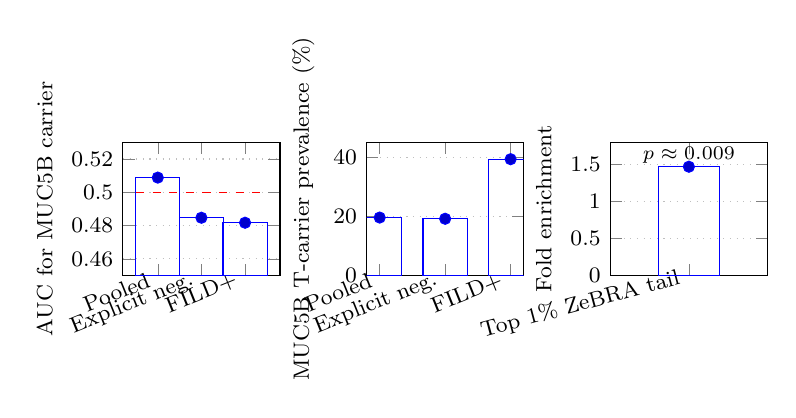
\begin{tikzpicture}
\begin{groupplot}[group style={group size=3 by 1,horizontal sep=1.1cm},width=0.295\textwidth,height=0.27\textwidth,tick label style={font=\footnotesize},label style={font=\footnotesize},ymajorgrids=true,major grid style={dotted}]
\nextgroupplot[ylabel={AUC for MUC5B carrier},ymin=0.45,ymax=0.53,xtick={0,1,2},xticklabels={Pooled,Explicit neg.,FILD+},xticklabel style={rotate=22,anchor=east}]
\addplot+[ybar,bar width=16pt] coordinates {(0,0.5088) (1,0.4847) (2,0.4817)};\addplot+[dashed,no marks] coordinates {(-0.5,0.5) (2.5,0.5)};
\nextgroupplot[ylabel={MUC5B T-carrier prevalence (\%)},ymin=0,ymax=45,xtick={0,1,2},xticklabels={Pooled,Explicit neg.,FILD+},xticklabel style={rotate=22,anchor=east}]
\addplot+[ybar,bar width=16pt] coordinates {(0,19.58) (1,19.17) (2,39.29)};
\nextgroupplot[ylabel={Fold enrichment},ymin=0,ymax=1.8,xtick={0},xticklabels={Top 1\% ZeBRA tail},xticklabel style={rotate=15,anchor=east}]
\addplot+[ybar,bar width=22pt] coordinates {(0,1.47)};\node[font=\scriptsize] at (axis cs:0,1.62) {$p\approx0.009$};
\end{groupplot}\end{tikzpicture}
\caption{The weak pooled ZeBRA--\textit{MUC5B} relationship is disease-mediated rather than genotype reconstruction. Left: ZeBRA-to-carrier AUC is at chance in pooled and FILD-stratified analyses. Middle: carrier prevalence is much higher among FILD/FILA-positive subjects. Right: the pooled extreme ZeBRA tail is modestly enriched for carriers.}
\label{fig:muc5b}
\end{figure*}

\subsection{Residual genomic information is localized}
The local-information analysis directly addresses the quantity suggested by Theorem~\ref{thm:main}(ii). Conditional \textit{MUC5B} evidence varies strongly across ZeBRA-defined control-FPR bands. In the 5--10\% band, the likelihood-ratio statistic for adding \textit{MUC5B} after ZeBRA is 16.55 ($p=4.74\times10^{-5}$); in the 20--40\% band it is 13.69 ($p=2.15\times10^{-4}$). This is not evidence that \textit{MUC5B} globally outperforms ZeBRA. It is evidence that residual genomic disease information is spatially heterogeneous in clinical-score space.

\begin{figure*}[!t]\centering\begin{tikzpicture}
\begin{groupplot}[group style={group size=2 by 1,horizontal sep=1.45cm},width=0.43\textwidth,height=0.28\textwidth,tick label style={font=\footnotesize},label style={font=\footnotesize},ymajorgrids=true,major grid style={dotted}]
\nextgroupplot[ylabel={Conditional MUC5B LRT after ZeBRA},ymin=0,ymax=19,xtick={1,2,3,4},xticklabels={2--5,5--10,10--20,20--40},xlabel={Control-FPR band (\%)}]
\addplot+[ybar,bar width=15pt] table[col sep=comma,x=band_index,y=lrt]{data/local_info_bands.csv};\addplot+[dashed,no marks] coordinates {(0.5,3.84) (4.5,3.84)};
\nextgroupplot[ylabel={Local ROC AUC},ymin=0.3,ymax=0.75,xtick={1,2,3,4},xticklabels={2--5,5--10,10--20,20--40},xlabel={Control-FPR band (\%)},legend style={at={(0.5,1.03)},anchor=south,legend columns=2,draw=none,font=\scriptsize}]
\addplot+[mark=*,thick] table[col sep=comma,x=band_index,y=auc_zebra]{data/local_info_bands.csv};\addlegendentry{ZeBRA}
\addplot+[mark=square*,thick] table[col sep=comma,x=band_index,y=auc_muc5b]{data/local_info_bands.csv};\addlegendentry{MUC5B}
\end{groupplot}\end{tikzpicture}
\caption{Localized genomic disease information. Left: conditional \textit{MUC5B} likelihood-ratio statistics after ZeBRA; the dashed line is the $\chi^2_1=3.84$ reference. Right: local discrimination varies by operating region, with \textit{MUC5B} stronger than ZeBRA in selected bands.}
\label{fig:local-info}
\end{figure*}

\begin{table*}[!t]\caption{Local FILD/FILA information in ZeBRA-defined control-FPR bands.}\label{tab:local-info}\centering\footnotesize
\begin{tabular}{lrrrrrr}\toprule
Band & $N$ & Cases & LRT $G\mid Z$ & $p$ & AUC ZeBRA & AUC \textit{MUC5B}\\\midrule
2--5\% & 401 & 26 & 4.44 & 0.0352 & 0.577 & 0.595\\
5--10\% & 652 & 26 & 16.55 & $4.74\times10^{-5}$ & 0.367 & 0.677\\
10--20\% & 1,281 & 30 & 4.77 & 0.0289 & 0.558 & 0.586\\
20--40\% & 2,540 & 37 & 13.69 & $2.15\times10^{-4}$ & 0.516 & 0.635\\\bottomrule
\end{tabular}\end{table*}

\subsection{Boundary-targeted genomics improves the operating decision}
A two-threshold rescue rule consults \textit{MUC5B} only for subjects lying between an upper and a lower ZeBRA threshold. Across all six evaluated threshold pairs, held-out sensitivity increases while realized overall FPR remains essentially unchanged. For the 0.5\%/10\% pair, sensitivity rises from 0.3587 to 0.4033 ($+0.0446$), FPR changes from 0.02335 to 0.02310, and LR$+$ increases from 15.58 to 17.54. This is the most direct empirical counterpart of boundary-localized utility.

\begin{figure*}[!t]\centering\begin{tikzpicture}
\begin{groupplot}[group style={group size=3 by 1,horizontal sep=1.1cm},width=0.30\textwidth,height=0.27\textwidth,tick label style={font=\footnotesize},label style={font=\footnotesize},ymajorgrids=true,major grid style={dotted}]
\nextgroupplot[ylabel={Held-out sensitivity},ymin=0.28,ymax=0.42,xtick={0,1,2,3,4,5},xticklabels={0.5/2,1/2,0.5/5,1/5,0.5/10,1/10},xticklabel style={rotate=34,anchor=east},xlabel={Upper/lower target FPR (\%)},legend style={at={(0.5,1.03)},anchor=south,legend columns=2,draw=none,font=\scriptsize}]
\addplot+[mark=*,thick] table[col sep=comma,x expr=\coordindex,y=zebra_sens]{data/boundary_rescue_summary_ordered_ext.csv};\addlegendentry{Matched ZeBRA}
\addplot+[mark=square*,thick] table[col sep=comma,x expr=\coordindex,y=rescue_sens]{data/boundary_rescue_summary_ordered_ext.csv};\addlegendentry{MUC5B rescue}
\nextgroupplot[xlabel={$\Delta$FPR},ylabel={$\Delta$sensitivity},xmin=-0.00032,xmax=0.00006,ymin=0,ymax=0.05,scaled x ticks=false,xtick={-0.0003,-0.0002,-0.0001,0},xticklabel style={/pgf/number format/fixed,/pgf/number format/precision=4,rotate=28,anchor=east}]
\addplot+[only marks,mark=*,mark size=2.4pt] table[col sep=comma,x=delta_fpr,y=delta_sens]{data/boundary_rescue_summary_ordered_ext.csv};\addplot+[dashed,no marks] coordinates {(-0.00032,0) (0.00006,0)};\addplot+[dashed,no marks] coordinates {(0,0) (0,0.05)};
\nextgroupplot[ylabel={LR$+$},ymin=12,ymax=42,xtick={0,1,2,3,4,5},xticklabels={0.5/2,1/2,0.5/5,1/5,0.5/10,1/10},xticklabel style={rotate=34,anchor=east},xlabel={Upper/lower target FPR (\%)}]
\addplot+[mark=*,thick] table[col sep=comma,x expr=\coordindex,y=zebra_lrplus]{data/boundary_rescue_summary_ordered_ext.csv};\addplot+[mark=square*,thick] table[col sep=comma,x expr=\coordindex,y=rescue_lrplus]{data/boundary_rescue_summary_ordered_ext.csv};
\end{groupplot}\end{tikzpicture}
\caption{Matched-FPR boundary rescue. Left: sensitivity of matched ZeBRA and boundary-targeted \textit{MUC5B} rescue. Center: every evaluated pair has positive sensitivity gain while $\Delta$FPR is near zero. Right: LR$+$ also increases under rescue.}
\label{fig:boundary-rescue}
\end{figure*}

\begin{table*}[!t]\caption{Selected matched-FPR boundary-rescue results over 100 repeated splits.}\label{tab:boundary-selected}\centering\footnotesize
\begin{tabular}{lrrrrrrrr}\toprule
Upper/lower & ZeBRA sens. & Rescue sens. & $\Delta$ sens. & ZeBRA FPR & Rescue FPR & ZeBRA LR$+$ & Rescue LR$+$ & Rescue LR$-$\\\midrule
1\%/5\% & 0.3303 & 0.3528 & +0.0225 & 0.01844 & 0.01826 & 18.19 & 19.52 & 0.659\\
0.5\%/5\% & 0.3121 & 0.3487 & +0.0366 & 0.01404 & 0.01400 & 22.74 & 25.21 & 0.661\\
1\%/10\% & 0.3740 & 0.4075 & +0.0335 & 0.02753 & 0.02735 & 13.75 & 14.95 & 0.609\\
0.5\%/10\% & 0.3587 & 0.4033 & +0.0446 & 0.02335 & 0.02310 & 15.58 & 17.54 & 0.611\\\bottomrule
\end{tabular}\end{table*}

\subsection{Low-FPR operating geometry}
The low-FPR view is most relevant to the clinical-tail part of the theorem. Across the evaluated matched operating points, rescue shifts sensitivity upward with very small FPR changes and systematically increases LR$+$. The pointwise envelope in Fig.~\ref{fig:low-fpr} is descriptive rather than a third classifier; it summarizes the best sensitivity achieved among the evaluated operating rules.

\begin{figure*}[!t]\centering\begin{tikzpicture}
\begin{groupplot}[group style={group size=2 by 1,horizontal sep=1.35cm},width=0.43\textwidth,height=0.29\textwidth,tick label style={font=\footnotesize},label style={font=\footnotesize},xmajorgrids=true,ymajorgrids=true,major grid style={dotted}]
\nextgroupplot[xlabel={False-positive rate},ylabel={Sensitivity},xmin=0,xmax=0.03,ymin=0.27,ymax=0.43,legend style={at={(0.5,1.03)},anchor=south,legend columns=3,draw=none,font=\scriptsize}]
\addplot+[only marks,mark=*,mark size=2.4pt] coordinates {(0.00801,0.2919) (0.01227,0.3046) (0.01404,0.3121) (0.01844,0.3303) (0.02335,0.3587) (0.02753,0.3740)};\addlegendentry{Matched ZeBRA}
\addplot+[only marks,mark=square*,mark size=2.4pt] coordinates {(0.00802,0.3101) (0.01228,0.3142) (0.01400,0.3487) (0.01826,0.3528) (0.02310,0.4033) (0.02735,0.4075)};\addlegendentry{MUC5B rescue}
\addplot+[dashed,thick,no marks] table[col sep=comma,x=fpr,y=tpr]{data/low_fpr_upper_envelope.csv};\addlegendentry{Pointwise envelope}
\nextgroupplot[xlabel={False-positive rate},ylabel={LR$+$},xmin=0.007,xmax=0.0285,ymin=12,ymax=42]
\addplot+[mark=*,thick] coordinates {(0.00801,38.16) (0.01227,25.43) (0.01404,22.74) (0.01844,18.19) (0.02335,15.58) (0.02753,13.75)};
\addplot+[mark=square*,thick] coordinates {(0.00802,39.67) (0.01228,26.03) (0.01400,25.21) (0.01826,19.52) (0.02310,17.54) (0.02735,14.95)};
\end{groupplot}\end{tikzpicture}
\caption{Low-FPR operating geometry. Boundary-targeted rescue occupies a favorable low-FPR region and increases LR$+$ without requiring improved global AUC.}
\label{fig:low-fpr}
\end{figure*}

\FloatBarrier
\section{Scope and limitations}

The theory is a statement about information channels, not about a particular machine-learning architecture. It does not require independence between genomics and clinical history; dependence is retained explicitly through $\LR_{G\mid C}$. It also applies to any deterministic genomic score derived from the measured genomic state through Corollary~2.

Several qualifications are essential. First, A1 is an explicit uniform boundedness assumption; non-Mendelian disease architecture motivates finite genomic evidence but does not prove a uniform bound after conditioning on every clinical state. Second, A2 is also an assumption. Sequential observations make likelihood-ratio accumulation possible, but high AUC alone does not establish an unbounded or sufficiently extended clinical tail. The empirical quantities most relevant to A2 are calibration, score-stratum likelihood ratios, stability of extreme-tail LR$+$, and fixed-specificity or partial-AUC behavior. Third, Theorem~\ref{thm:main}(ii) concerns threshold changes, not posterior-probability changes: genomics may still shift posterior risk away from the boundary even when it cannot reverse the decision. Fourth, the operational FILD/FILA target in the historical notebook construction maps missing adjudication values to zero; consequently, the target-zero group should not be described as a fully adjudicated control cohort without further confirmation. Finally, the particular genomic rescue rule remains a modeling result that requires independent or prospectively prespecified validation. The empirical analyses support the predicted geometry but do not validate A1 or A2 by themselves.

A stronger future validation of the theory should therefore test ZeBRA calibration, convert score strata into empirical likelihood ratios, quantify uncertainty in extreme-tail LR$+$, evaluate prespecified fixed-specificity thresholds, and replicate boundary-localized genomic rescue in an external cohort.

\section{Conclusion}

The central result is not that clinical history ``contains'' genomics, nor that genomics is globally useless. The two modalities are distinct evidence channels. Bayes' rule factorizes their joint evidence into a clinical likelihood ratio and a residual genomic likelihood ratio conditional on clinical state. If the residual genomic factor is bounded while sequential clinical evidence can extend into a strong likelihood-ratio tail, then genomic information can reverse a clinical threshold decision only inside a bounded neighborhood of that threshold, and sufficiently extreme clinical evidence must eventually dominate every bounded genomic-only rule. Any deterministic genomic predictor inherits the same finite-evidence constraint, while Proposition~\ref{prop:auc-local} explains why clinically meaningful boundary reclassification can coexist with almost no change in global AUC.

The current Colorado results match this qualitative geometry. ZeBRA dominates global discrimination; broad genomic augmentation provides essentially zero incremental FILD/FILA AUC after conditioning on ZeBRA; ZeBRA does not reconstruct \textit{MUC5B}; residual \textit{MUC5B} disease information is concentrated in selected ZeBRA operating bands; and a boundary-targeted rescue rule improves sensitivity and LR$+$ at essentially matched overall FPR. The resulting picture is one of \emph{regime-dependent complementarity}: genomics is most useful where the clinical evidence is close enough to the action threshold that a finite residual Bayes factor can still change the decision, whereas longitudinal clinical evidence dominates in the extreme tail.

\begin{thebibliography}{99}

\bibitem{Onishchenko2026}
D.~Onishchenko, J.~A. Mastrianni, and I.~Chattopadhyay,
``Passive early screening for Alzheimer's disease and related dementias using EHR comorbidity patterns,''
\emph{npj Digital Medicine}, vol.~9, 2026, doi: 10.1038/s41746-026-02954-2.

\bibitem{Seibold2011}
M.~A. Seibold \emph{et al.},
``A common \textit{MUC5B} promoter polymorphism and pulmonary fibrosis,''
\emph{New England Journal of Medicine}, vol.~364, no.~16, pp.~1503--1512, 2011, doi: 10.1056/NEJMoa1013660.

\bibitem{Fingerlin2013}
T.~E. Fingerlin \emph{et al.},
``Genome-wide association study identifies multiple susceptibility loci for pulmonary fibrosis,''
\emph{Nature Genetics}, vol.~45, no.~6, pp.~613--620, 2013, doi: 10.1038/ng.2609.

\bibitem{Allen2020}
R.~J. Allen \emph{et al.},
``Genome-wide association study of susceptibility to idiopathic pulmonary fibrosis,''
\emph{American Journal of Respiratory and Critical Care Medicine}, vol.~201, no.~5, pp.~564--574, 2020, doi: 10.1164/rccm.201905-1017OC.

\bibitem{NeymanPearson1933}
J.~Neyman and E.~S. Pearson,
``On the problem of the most efficient tests of statistical hypotheses,''
\emph{Philosophical Transactions of the Royal Society of London. Series A}, vol.~231, pp.~289--337, 1933, doi: 10.1098/rsta.1933.0009.

\bibitem{Wald1945}
A.~Wald,
``Sequential tests of statistical hypotheses,''
\emph{The Annals of Mathematical Statistics}, vol.~16, no.~2, pp.~117--186, 1945.

\bibitem{CoverThomas2006}
T.~M. Cover and J.~A. Thomas,
\emph{Elements of Information Theory}, 2nd~ed.
Hoboken, NJ, USA: Wiley, 2006.

\end{thebibliography}

\end{document}
